\usetikzlibrary{arrows.meta,fit}
\begin{frame}[plain]{pa = translate(va) [LEVELS=2]}
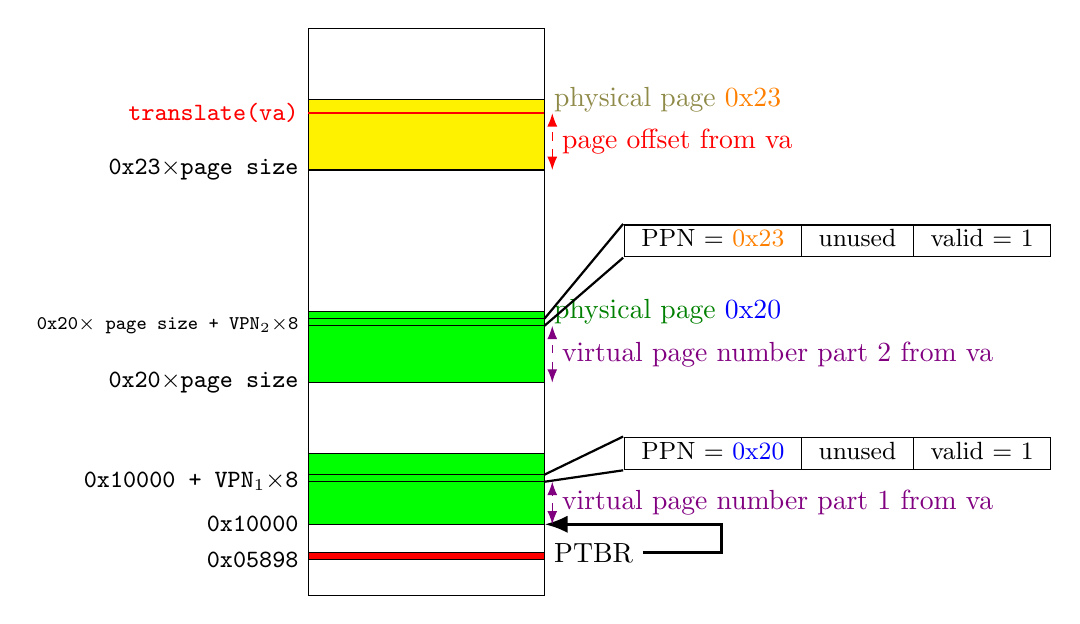
\begin{tikzpicture}
\tikzset{
    y=0.9cm
}
\draw (0, 0) rectangle (3, -8);
\draw[fill=red] (0, -7.5) rectangle (3, -7.4)
    node[right] (ptbr) {PTBR};
\draw[fill=green] (0, -6) rectangle (3, -7);
\draw[-Latex, very thick] (ptbr.east) -- ++(1cm, 0cm) |- (3, -7);
\node[font=\small\tt,anchor=east] at (0, -7.5) {0x05898};
\node[font=\small\tt,anchor=east] at (0, -7) {0x10000};
\node[font=\small\tt,anchor=east] at (0, -6.4) {0x10000 + $\text{\tt VPN}_1\times$8};
\node[font=\small\tt,anchor=east] at (0, -5) {0x20$\times$page size};
\node[font=\small\tt,anchor=east,align=right] at (0, -4.2) {\scriptsize 0x20$\times$ page size + $\text{\tt VPN}_2\times$8};
\node[font=\small\tt,anchor=east] at (0, -2) {0x23$\times$page size};

\draw[fill=green] (0, -5) rectangle (3, -4)
    node[right,yshift=-0cm,green!50!black] {physical page {\color{blue}0x20}};
\draw[fill=yellow] (0, -2) rectangle (3, -1)
    node[right,yshift=-0cm,yellow!50!black] {physical page {\color{orange}0x23}};
\draw[Latex-Latex,violet,dashed] (3.1, -7) -- (3.1, -6.4) node[midway,right] {virtual page number part 1 from va};
\draw (0, -6.4) rectangle (3, -6.3);
\node[anchor=west,font=\small,inner sep=0mm] (pte) at (4, -6) {
    \begin{tabular}{|l|l|l|} \hline
    PPN = {\color{blue}0x20} & unused & valid = 1 \\ \hline
    \end{tabular}
};
\draw[thick] (3, -6.4) -- (pte.south west);
\draw[thick] (3, -6.3) -- (pte.north west);

\draw[Latex-Latex,violet,dashed] (3.1, -5) -- (3.1, -4.2) node[midway,right]  {virtual page number part 2 from va};
\draw (0, -4.2) rectangle (3, -4.1);
\node[anchor=west,font=\small,inner sep=0mm] (pte 2) at (4, -3) {
    \begin{tabular}{|l|l|l|} \hline
    PPN = {\color{orange}0x23} & unused & valid = 1 \\ \hline
    \end{tabular}
};
\draw[thick] (3, -4.2) -- (pte 2.south west);
\draw[thick] (3, -4.1) -- (pte 2.north west);

\draw[Latex-Latex,red,dashed] (3.1, -2) -- (3.1, -1.2) node[midway, right] {page offset from va};
\draw[thick,red] (0, -1.2) -- (3, -1.2);

\node[red,font=\small\tt,anchor=east] at (0, -1.2) {translate(va)};

\end{tikzpicture}
\end{frame}

\usetikzlibrary{arrows.meta,fit}
\begin{frame}[plain]{first page\_allocate(va) [LEVELS=2]}
\begin{tikzpicture}
\tikzset{
    y=0.9cm
}
\draw (0, 0) rectangle (3, -8);
\draw[fill=red] (0, -7.5) rectangle (3, -7.4)
    node[right] (ptbr) {PTBR};
\begin{visibleenv}<2->
\draw[fill=green] (0, -6) rectangle (3, -7);
\draw[-Latex, very thick,alt=<2>{red}] (ptbr.east) -- ++(1cm, 0cm) |- (3, -7);
\end{visibleenv}
\node[font=\small\tt,anchor=east] at (0, -7.5) {0x05898};
\begin{visibleenv}<3->
\node[font=\small\tt,anchor=east] at (0, -7) {NEW0};
\node[font=\small\tt,anchor=east] at (0, -6.4) {NEW0 + $\text{\tt VPN}_1\times$8};
\end{visibleenv}
\begin{visibleenv}<4->
\node[font=\small\tt,anchor=east] at (0, -5) {NEW1$\times$page size};
\node[font=\small\tt,anchor=east,align=right] at (0, -4.2) {\scriptsize NEW1$\times$ page size + $\text{\tt VPN}_2\times$8};
\end{visibleenv}
\begin{visibleenv}<5->
\node[font=\small\tt,anchor=east] at (0, -2) {NEW2$\times$page size};
\end{visibleenv}

\begin{visibleenv}<4->
\draw[fill=green] (0, -5) rectangle (3, -4)
    node[right,yshift=-0cm,green!50!black] {physical page {\color{blue}NEW1}};
\end{visibleenv}
\begin{visibleenv}<5->
\draw[fill=yellow] (0, -2) rectangle (3, -1)
    node[right,yshift=-0cm,yellow!50!black] {physical page {\color{orange}NEW2}};
\end{visibleenv}
\begin{visibleenv}<2->
\draw[Latex-Latex,violet,dashed] (3.1, -7) -- (3.1, -6.4) node[midway,right] {virtual page number part 1 from va};
\draw (0, -6.4) rectangle (3, -6.3);
\node[anchor=west,font=\small,inner sep=0mm,alt=<2>{fill=red!10}] (pte) at (4, -6) {
    \begin{tabular}{|l|l|l|} \hline
    PPN = \alt<3->{\color{blue}NEW1}{---} & unused & valid = \alt<3->{1}{0} \\ \hline
    \end{tabular}
};
\draw[thick] (3, -6.4) -- (pte.south west);
\draw[thick] (3, -6.3) -- (pte.north west);
\end{visibleenv}

\begin{visibleenv}<3->
\draw[Latex-Latex,violet,dashed] (3.1, -5) -- (3.1, -4.2) node[midway,right]  {virtual page number part 2 from va};
\draw (0, -4.2) rectangle (3, -4.1);
    \node[anchor=west,font=\small,inner sep=0mm,alt=<4>{fill=red!10}] (pte 2) at (4, -3) {
    \begin{tabular}{|l|l|l|} \hline
        PPN = \alt<4->{\color{orange}NEW2}{---} & unused & valid = \alt<4->{1}{0} \\ \hline
    \end{tabular}
};
\draw[thick] (3, -4.2) -- (pte 2.south west);
\draw[thick] (3, -4.1) -- (pte 2.north west);
\end{visibleenv}

\begin{visibleenv}<5->
\draw[Latex-Latex,red,dashed] (3.1, -2) -- (3.1, -1.2) node[midway, right] {page offset from va};
\draw[thick,red] (0, -1.2) -- (3, -1.2);

\node[red,font=\small\tt,anchor=east] at (0, -1.2) {translate(va)};
\end{visibleenv}
\end{tikzpicture}
\end{frame}

\begin{frame}{later page allocates?}
    \begin{itemize}
    \item some of those allocations done earlier
        \begin{itemize}
        \item e.g. ptbr already set
        \end{itemize}
    \item should reuse existing allocation then
    \end{itemize}
\end{frame}
